\chapter{A Salvação de Deus: a Lei e a Graça}

Chamado à bem-aventurança, mas ferido pelo pecado, o homem tem necessidade da salvação de Deus. O auxílio divino é-lhe dado em Cristo, pela lei que o dirige e pela graça que o ampara: ``Trabalhai com temor e tremor na vossa salvação: porque é Deus que opera em vós o querer e o agir, segundo os seus desígnios'' (Fl 2,12--13). Nos parágrafos 1949 a 2051, o Catecismo da Igreja Católica apresenta os dois grandes instrumentos pelos quais Deus conduz o homem ao seu fim último: a lei moral, que ilumina o caminho, e a graça, que dá a força para percorrê-lo. Não se trata de dois poderes concorrentes, mas de dois dons do mesmo amor divino: a lei sem a graça seria letra morta, e a graça sem a lei seria uma força sem direção. Juntos, lei e graça configuram o homem a Cristo e o habilitam a \textbf{fazer o bem} em plenitude.

\section{A lei moral (1950--1986)}

A lei moral é obra da Sabedoria divina. Pode definir-se, em sentido bíblico, como uma instrução paterna, uma pedagogia de Deus: ela prescreve ao homem os caminhos, as regras de procedimento que o levam à bem-aventurança prometida e lhe proíbe os caminhos do mal, que desviam de Deus e do seu amor. A lei é ``uma regra de procedimento emanada da autoridade competente em ordem ao \textbf{bem} comum''; a lei moral pressupõe a ordem racional estabelecida entre as criaturas para o seu \textbf{bem} e em vista do seu fim, pelo poder, sabedoria e bondade do Criador. ``Esta ordenação da razão, eis o que se chama a lei'' (São Tomás de Aquino). As expressões da lei moral são diversas, mas todas coordenadas entre si --- a lei eterna, a lei natural, a lei revelada (compreendendo a Lei antiga e a Lei nova ou evangélica) e, por fim, as leis civis e eclesiásticas ---, tendo em Cristo a sua plenitude e unidade: ``O fim da Lei é Cristo, para a justificação de todo o crente'' (Rm 10,4).

O homem participa na sabedoria e na bondade do Criador, que lhe confere o domínio dos seus atos e a capacidade de se governar em ordem à verdade e ao \textbf{bem}. A lei natural exprime o sentido moral original que permite ao homem discernir, pela razão, o \textbf{bem} e o mal: está ``escrita e gravada na alma de todos e de cada um dos homens, porque não é senão a razão humana ordenando \textbf{fazer o bem} e proibindo pecar'' (Leão XIII, \textit{Libertas praestantissimum}). Esta lei divina e natural mostra ao homem o caminho a seguir para praticar o \textbf{bem} e atingir o seu fim; tem como fulcro a aspiração e a submissão a Deus, ``fonte e juiz de todo o \textbf{bem}'', e o sentido do outro como igual a si mesmo. A lei natural é universal nos seus preceitos, imutável e permanente através das variações da história; subsiste sob o fluxo das ideias e dos costumes, e ``mesmo que se lhe neguem até os princípios, não é possível destruí-la nem tirá-la do coração do homem: ela ressurge sempre na vida dos indivíduos e das sociedades''. A Lei antiga, por sua vez, foi o primeiro estádio da lei revelada, cujas prescrições morais estão compendiadas nos Dez Mandamentos: proibem o que é contrário ao amor de Deus e do próximo e prescrevem o que lhe é essencial; são uma ``luz oferecida à consciência de todo o homem''. A Lei antiga é, porém, imperfeita: como pedagogia, mostra o que se deve fazer, mas por si não dá a força, a graça do Espírito para ser cumprida; tem por função principal denunciar e manifestar o pecado, preparando e dispondo para a conversão e para a fé em Deus salvador.

A Lei nova ou Lei evangélica é a perfeição, na terra, da Lei divina, natural e revelada. É obra de Cristo e tem a sua expressão de modo particular no Sermão da Montanha; é também obra do Espírito Santo e, por Ele, torna-se a lei interior da caridade: ``Hei-de imprimir as minhas leis no seu espírito e gravá-las-ei no seu coração'' (Heb 8,10). A Lei nova é a graça do Espírito Santo, dada pelos fiéis pela fé em Cristo; opera pela caridade e serve-se do Sermão do Senhor para nos ensinar o que se deve fazer, e dos sacramentos para nos comunicar a graça de o fazer. Ela cumpre, apura, ultrapassa e leva à perfeição a Lei antiga: nas bem-aventuranças, cumpre as promessas divinas; e, longe de abolir as prescrições morais da Lei antiga, tira delas as virtualidades ocultas, chegando a reformar a raiz dos atos, o coração, onde o homem escolhe entre o puro e o impuro, onde se formam a fé, a esperança e a caridade e, com elas, as outras virtudes. A Lei nova resume-se na regra de ouro: ``Tudo quanto quiserdes que os homens vos façam, fazei-lho, de igual modo, vós também'' (Mt 7,12); e apoia-se toda no ``mandamento novo'' de Jesus, de nos amarmos uns aos outros como Ele nos amou (cf.~Jo 15,12). É chamada lei do amor, porque faz agir mais pelo amor infundido pelo Espírito Santo do que pelo temor; lei da graça, porque confere a força da graça para agir pela fé e pelos sacramentos; e lei de liberdade, porque nos liberta das observâncias rituais e jurídicas da Lei antiga, nos inclina a agir espontaneamente sob o impulso da caridade e nos faz passar da condição do escravo para a do amigo de Cristo e do filho herdeiro. Além dos seus preceitos, a Lei nova inclui também os conselhos evangélicos, que manifestam a plenitude viva da caridade, sempre insatisfeita por não dar mais.

\begin{figure}[htbp]
    \centering
    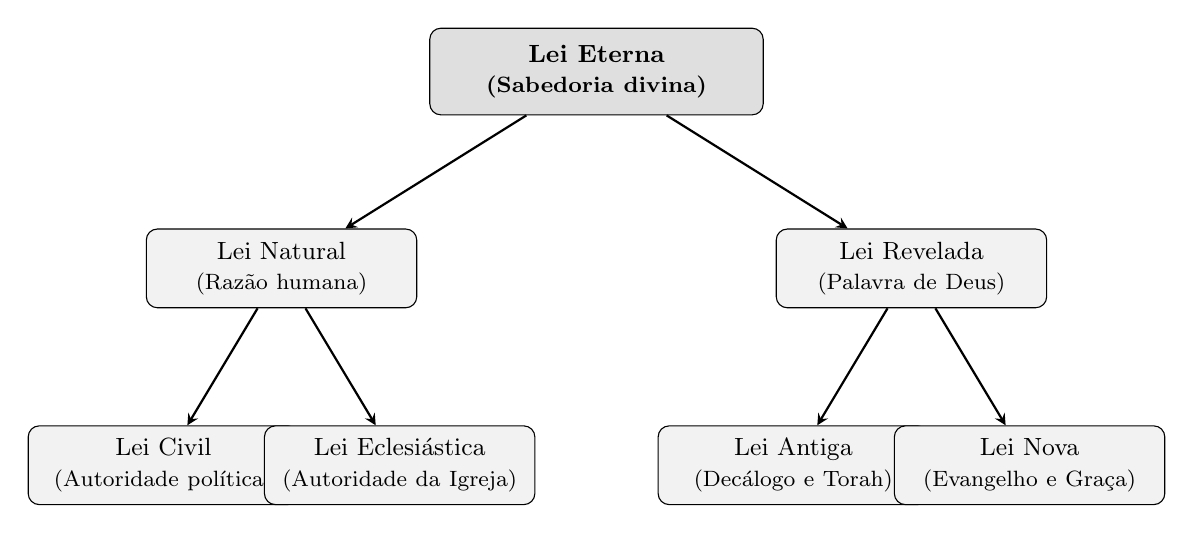
\begin{tikzpicture}[
            every node/.style={font=\small},
            boxstyle/.style={
                    draw, rounded corners=4pt,
                    text centered, text width=3.2cm,
                    minimum height=1.0cm,
                    fill=gray!10
                },
            rootstyle/.style={
                    draw, rounded corners=4pt,
                    text centered, text width=4.0cm,
                    minimum height=1.1cm,
                    fill=gray!25, font=\small\bfseries
                },
            arrow/.style={->, >=stealth, thick}
        ]

        % Raiz
        \node[rootstyle] (eternal) at (0,0) {Lei Eterna\\{\footnotesize(Sabedoria divina)}};

        % Segundo nível
        \node[boxstyle] (natural) at (-4,-2.5) {Lei Natural\\{\footnotesize(Razão humana)}};
        \node[boxstyle] (revealed) at (4,-2.5) {Lei Revelada\\{\footnotesize(Palavra de Deus)}};

        % Terceiro nível — lei natural
        \node[boxstyle] (civil) at (-5.5,-5.0) {Lei Civil\\{\footnotesize(Autoridade política)}};
        \node[boxstyle] (eccl) at (-2.5,-5.0) {Lei Eclesiástica\\{\footnotesize(Autoridade da Igreja)}};

        % Terceiro nível — lei revelada
        \node[boxstyle] (old) at (2.5,-5.0) {Lei Antiga\\{\footnotesize(Decálogo e Torah)}};
        \node[boxstyle] (new) at (5.5,-5.0) {Lei Nova\\{\footnotesize(Evangelho e Graça)}};

        % Setas
        \draw[arrow] (eternal) -- (natural);
        \draw[arrow] (eternal) -- (revealed);

        \draw[arrow] (natural) -- (civil);
        \draw[arrow] (natural) -- (eccl);

        \draw[arrow] (revealed) -- (old);
        \draw[arrow] (revealed) -- (new);

    \end{tikzpicture}
    \caption{Hierarquia das leis segundo o Catecismo da Igreja Católica (\S\S 1950--1952)}
    \label{fig:hierarquia-leis}
\end{figure}

\section{Graça e justificação (1987--2029)}

A graça do Espírito Santo tem o poder de nos justificar, isto é, de nos lavar dos nossos pecados e de nos comunicar ``a justiça de Deus pela fé em Jesus Cristo'' e pelo Batismo (cf.~Rm 3,22; 6,3--4). Pelo poder do Espírito Santo, tomamos parte na paixão de Cristo, morrendo para o pecado, e na sua ressurreição, nascendo para uma vida nova; somos os membros do seu corpo, que é a Igreja, e os sarmentos enxertados na videira que é Ele próprio. A primeira obra da graça do Espírito Santo é a conversão, que opera a justificação: sob a moção da graça, o homem volta-se para Deus e desvia-se do pecado, acolhendo o perdão e a justiça do Alto. ``A justificação comporta, portanto, a remissão dos pecados, a santificação e a renovação do homem interior'' (Concílio de Trento). A justificação desliga o homem do pecado, reconcilia-o com Deus e liberta-o da escravidão do pecado; foi merecida pela paixão de Cristo, que na cruz se ofereceu como hóstia viva, santa e agradável a Deus, e é concedida pelo Batismo, sacramento da fé. A justificação estabelece também a colaboração entre a graça de Deus e a liberdade do homem: ``quando Deus move o coração do homem pela iluminação do Espírito Santo, o homem não fica sem fazer nada ao receber esta inspiração'' (Concílio de Trento); no entanto, também não pode, sem a graça de Deus, caminhar por sua livre vontade para a justiça na sua presença. ``A justificação é a obra mais excelente do amor de Deus manifestado em Cristo Jesus e concedido pelo Espírito Santo'' (cf. Santo Agostinho); pensa mesmo que ``a justificação do ímpio é obra maior que a criação do céu e da terra'', porque ``o céu e a terra passarão, ao passo que a justificação e a salvação dos eleitos permanecerão''.

A nossa justificação vem da graça de Deus. A graça é o favor, o socorro gratuito que Deus nos dá, a fim de respondermos ao seu chamamento para nos tornarmos filhos de Deus, filhos adotivos, participantes da natureza divina e da vida eterna. É uma participação na vida de Deus que nos introduz na intimidade da vida trinitária: pelo Batismo, o cristão participa na graça de Cristo, cabeça do seu corpo; como filho adotivo, pode chamar ``Pai'' a Deus; e recebe a vida do Espírito, que lhe infunde a caridade e forma a Igreja. Esta vocação é sobrenatural e depende inteiramente da iniciativa gratuita de Deus, pois só Ele pode revelar-Se e dar-Se a Si mesmo. A graça santificante é um dom habitual, uma disposição estável e sobrenatural que aperfeiçoa a alma para a tornar capaz de viver com Deus e de agir por seu amor. A preparação do homem para acolher a graça é já obra da graça: ``é Ele próprio que começa, fazendo com que queiramos, e é Ele que acaba, cooperando com aqueles que assim querem'' (Santo Agostinho). A graça compreende ainda os dons que o Espírito dá para nos associar à sua obra --- as graças sacramentais, próprias dos diferentes sacramentos, e as graças especiais ou carismas, ordenados para o \textbf{bem} comum da Igreja e ao serviço da caridade que a edifica.

O mérito do homem perante Deus, na vida cristã, provém do facto de que Deus dispôs livremente associar o homem à obra da sua graça. O mérito pertence, em primeiro lugar, à graça de Deus; o próprio mérito do homem depende d'Ele, porque as suas boas ações procedem, em Cristo, das predisposições e ajudas do Espírito Santo. ``Quando coroais os seus méritos, coroais os vossos próprios dons'' (Prefácio dos Santos). A adoção filial pode conferir-nos, segundo a justiça gratuita de Deus, um verdadeiro mérito: ``Os méritos das nossas boas obras são dons da bondade divina. Os méritos são dons de Deus'' (Santo Agostinho). Uma vez que a iniciativa pertence a Deus, ninguém pode merecer a graça primeira, que está na origem da conversão. Mas, sob a moção do Espírito Santo e da caridade, podemos merecer para nós mesmos e para outros as graças úteis para a santificação, para o aumento da graça e da caridade, bem como para a obtenção da vida eterna. Os cristãos de qualquer estado ou ordem são chamados à plenitude da vida cristã e à perfeição da caridade: ``Sede perfeitos, como o vosso Pai celeste é perfeito'' (Mt 5,48). O caminho desta perfeição passa pela cruz, pois ``não há santidade sem renúncia e combate espiritual''; mas é caminho de esperança: ``os filhos da santa Igreja, nossa Mãe, esperam justamente a graça da perseverança final e a recompensa de Deus seu Pai pelas boas obras realizadas com a sua graça, em comunhão com Jesus''.

\section{A Igreja, mãe e educadora (2030--2051)}

É em Igreja, em comunhão com todos os batizados, que o cristão realiza a sua vocação. Da Igreja recebe a Palavra de Deus, que contém os ensinamentos da ``lei de Cristo'' (Gl 6,2); da Igreja recebe a graça dos sacramentos que o sustentam no caminho; e da Igreja recebe o exemplo da santidade, cujo modelo e fonte é a Santíssima Virgem Maria. A vida moral é um culto espiritual: nós ``oferecemos os nossos corpos como sacrifício vivo, santo, agradável a Deus'' (Rm 12,1), no seio do corpo de Cristo que formamos e em comunhão com a oferenda da sua Eucaristia. Como todo o conjunto da vida cristã, a vida moral tem a sua fonte e o seu ponto alto no sacrifício eucarístico. A Igreja, ``coluna e fundamento da verdade'' (1 Tm 3,15), recebeu dos Apóstolos o solene mandamento de Cristo de anunciar a verdade da salvação; ``à Igreja compete anunciar sempre e em toda a parte os princípios morais, mesmo de ordem social, bem como emitir juízo acerca de quaisquer realidades humanas, na medida em que o exigirem os direitos fundamentais da pessoa humana ou a salvação das almas'' (CIC, can. 747 §2).

O Magistério dos pastores da Igreja exerce-se ordinariamente na catequese e na pregação, com a ajuda das obras dos teólogos e autores espirituais. O Romano Pontífice e os bispos, como ``doutores autênticos, investidos na autoridade de Cristo, pregam ao povo a eles confiado a fé que deve ser acreditada e aplicada nos costumes'' (LG 25); ensinam a verdade que se deve crer, a caridade que se deve praticar e a bem-aventurança que se deve esperar. A autoridade do Magistério estende-se também aos preceitos específicos da lei natural, porque a sua observância, exigida pelo Criador, é necessária à salvação. A Lei de Deus, confiada à Igreja, é ensinada aos fiéis como caminho de vida e de verdade; os fiéis têm o direito de serem instruídos sobre os preceitos divinos salvíficos que purificam o juízo, e o dever de observar as constituições e decretos emanados da autoridade legítima da Igreja. A consciência de cada um deve abrir-se o mais possível ``à consideração do \textbf{bem} de todos, tal como ele se exprime na lei moral, natural e revelada, e consequentemente, na lei da Igreja e no ensino autorizado do Magistério sobre as questões morais''; não convém opor a consciência pessoal e a razão à lei moral ou ao Magistério. Pode desenvolver-se assim entre os cristãos um verdadeiro espírito filial em relação à Igreja: a Igreja concede-nos a misericórdia de Deus, que supera todos os nossos pecados, e administra-nos na sua liturgia o alimento da Palavra e da Eucaristia do Senhor.

\subsection*{Os Mandamentos da Igreja}

Os preceitos da Igreja inserem-se na linha de uma vida moral ligada à vida litúrgica e nutrindo-se dela. O caráter obrigatório destas leis positivas, promulgadas pelas autoridades pastorais, tem por fim garantir aos fiéis ``o mínimo indispensável de espírito de oração e de esforço moral e de crescimento no amor a Deus e ao próximo''. Tradição catequética enumera habitualmente cinco preceitos gerais da Igreja:

\begin{description}

    \item[Primeiro preceito: Santificar os domingos e as festas de guarda.] Os fiéis são obrigados a participar na Missa nos domingos e nos outros dias santos de obrigação e a abster-se dos trabalhos e ocupações que possam impedir a santificação desses dias, a alegria própria do Dia do Senhor ou o descanso conveniente do espírito e do corpo. O domingo, ``dia da ressurreição do Senhor'', é o primordial dia santo de obrigação. São também dias santos de obrigação, além do domingo: a Natividade do Senhor, a Epifania, a Ascensão, o Corpo e Sangue de Cristo, a Solenidade de Santa Maria Mãe de Deus, a Imaculada Conceição, a Assunção, São José, São Pedro e São Paulo e Todos os Santos (cf.~CIC, can. 1246--1248; CCEO, can. 880--881). ``Participar na Missa'' inclui assistir a qualquer celebração eucarística em rito católico, quer no próprio dia quer na tarde/noite do dia anterior. Se a participação na Eucaristia for impossível por ausência de ministro sagrado ou outra causa grave, recomenda-se vivamente que os fiéis se dediquem à liturgia da Palavra ou à oração em família (cf.~CIC, can. 1248 §2).

    \item[Segundo preceito: Confessar os pecados graves ao menos uma vez por ano.] Depois de atingir a idade do discernimento, cada fiel é obrigado a confessar fielmente os seus pecados graves ao menos uma vez por ano (cf.~CIC, can. 989). Este preceito assegura a preparação para a Eucaristia mediante a recepção do sacramento da Reconciliação, que continua a obra de conversão e perdão do Batismo. Ao sacramento da Penitência se une também, no contexto da vida sacramental ordinária, o discernimento da própria consciência à luz da lei de Deus.

    \item[Terceiro preceito: Comungar ao menos na Páscoa da Ressurreição.] Iniciada na Eucaristia, cada pessoa é obrigada a receber a Sagrada Comunhão ao menos uma vez por ano, preferencialmente durante o tempo pascal (cf.~CIC, can. 920). Este preceito garante um mínimo na recepção do Corpo e Sangue do Senhor, em ligação com as festas pascais, que são a origem e o centro da liturgia cristã. O preceito pode ser cumprido em outro tempo do ano por causa justa.

    \item[Quarto preceito: Guardar abstinência e jejuar nos dias determinados pela Igreja.] A lei divina obriga todos os fiéis a \textbf{fazer penitência}, cada um à sua maneira. Para que haja também uma observância comum, o Código de Direito Canônico estabelece dias penitenciais, em que os fiéis se dedicam de modo especial à oração, a obras de piedade e caridade, e praticam o jejum e a abstinência (cf.~CIC, can. 1249--1251; CCEO, can. 882). Estes dias de ascese ``contribuem para nos fazer adquirir domínio sobre os nossos instintos e a liberdade do coração''. As conferências episcopais podem determinar, com maior particularidade, os modos de observância penitencial para o seu território.

    \item[Quinto preceito: Prover às necessidades materiais da Igreja.] Os fiéis têm a obrigação de prover às necessidades materiais da Igreja consoante as possibilidades de cada um (cf.~CIC, can. 222; CCEO, can. 25), contribuindo para a sustentação dos ministérios, das obras de culto e da caridade eclesial. Este preceito enraíza-se no princípio de que a comunidade eclesial, como qualquer comunidade humana, necessita de recursos para cumprir a sua missão. As Conferências Episcopais podem, para além destes cinco preceitos gerais, estabelecer outros preceitos eclesiásticos para o seu território (cf.~CIC, can. 455).

\end{description}

A fidelidade dos batizados na observância destes preceitos é condição primordial para o anúncio do Evangelho e para a missão da Igreja no mundo: ``O testemunho de vida cristã e as obras realizadas com espírito sobrenatural são meios poderosos para atrair os homens à fé e a Deus'' (AA 6). Os cristãos contribuem, pela constância das suas convicções e dos seus costumes, para a edificação da Igreja; e, vivendo segundo Cristo, apressam a vinda do Reino de Deus, do ``Reino da justiça, da verdade e da paz'', cumprindo com retidão, paciência e amor as suas tarefas terrestres.

\section{Os dez mandamentos (2052--2082)}

«Mestre, que devo fazer de \textbf{bem} para ter a vida eterna?» Ao jovem que Lhe faz esta pergunta, Jesus responde, primeiro, invocando a necessidade de reconhecer a Deus como «o único \textbf{Bem}, o \textbf{Bem} por excelência e a fonte de todo o \textbf{bem}». Depois declara-lhe: «Se queres entrar na vida, observa os mandamentos». E cita os mandamentos que dizem respeito ao amor do próximo, resumindo-os de modo positivo: «Amarás o teu próximo como a ti mesmo» (Mt 19,16-19). A esta primeira resposta vem juntar-se uma segunda, o convite à perfeição: «Se queres ser perfeito, vai, vende os teus \textbf{bens} e dá-os aos pobres, e terás um tesouro nos céus. Vem, depois, e segue-Me» (Mt 19,21); mas esta segunda resposta não anula a primeira, pois seguir Jesus implica cumprir os mandamentos --- a Lei não é abolida, mas o homem é convidado a reencontrá-la na Pessoa do seu Mestre, em Quem ela encontra o seu perfeito cumprimento. Jesus retomou os dez mandamentos, mas manifestou a força do Espírito que atua na letra em que eles se exprimem: pregou a «justiça que excede a dos escribas e fariseus» e explicou todas as exigências dos mandamentos, chegando à sua raiz interior. Perguntado qual é o maior mandamento da Lei, Jesus responde: «Amarás o Senhor teu Deus, com todo o teu coração, com toda a tua alma e com toda a tua mente: tal é o maior e primeiro mandamento. O segundo é semelhante a este: Amarás o teu próximo como a ti mesmo. A estes dois mandamentos está ligada toda a Lei, bem como os Profetas» (Mt 22,37-40). O Decálogo deve ser interpretado à luz deste duplo e único mandamento da caridade, plenitude da Lei: «O amor não faz mal ao próximo. Assim, é no amor que está o pleno cumprimento da Lei» (Rm 13,9-10).

A palavra «Decálogo» significa literalmente «dez palavras», reveladas por Deus ao seu povo na montanha sagrada e escritas com o «seu Dedo» (cf.~Ex 31,18), diferentemente dos outros preceitos escritos por Moisés. O Decálogo compreende-se, antes de mais nada, no contexto do Êxodo --- o grande acontecimento libertador de Deus, no centro da Antiga Aliança. Quer formuladas como preceitos negativos ou como mandamentos positivos, as «dez palavras» indicam as condições de uma vida liberta da escravidão do pecado: «Se amares o teu Deus, andares nos seus caminhos e guardares os seus mandamentos, leis e costumes, viverás e multiplicar-te-ás» (Dt 30,16). Pronunciadas por Deus no decurso de uma teofania, elas fazem parte da revelação que Ele fez de Si mesmo e da sua glória: «o dom dos mandamentos é uma dádiva do próprio Deus e da sua santa vontade». É no âmbito da Aliança que os mandamentos recebem o seu pleno significado: a existência moral é resposta à iniciativa amorosa do Senhor, é reconhecimento, homenagem a Deus e culto de ação de graças, é cooperação com o plano que Deus prossegue na história. Ao mesmo tempo que a todo o povo, Deus faz conhecer a sua vontade a cada um em particular: «O Senhor prescreveu o amor para com Deus e ensinou a justiça para com o próximo, para que o homem não fosse nem injusto nem indigno de Deus. Assim, através do Decálogo, Deus preparava o homem para se tornar seu amigo e ter um só coração com o seu próximo» (Santo Ireneu de Lião, \textit{Adversus haereses}).

Na fidelidade à Sagrada Escritura e em conformidade com o exemplo de Jesus, a Tradição da Igreja reconheceu no Decálogo uma importância e um significado primordiais. Desde Santo Agostinho, os «Dez Mandamentos» ocupam lugar preponderante na catequese dos futuros batizados e dos fiéis; os catecismos da Igreja expuseram muitas vezes a moral cristã seguindo a ordem dos «Dez Mandamentos». O Decálogo forma um todo indissociável: cada «Palavra» remete para cada uma das outras; elas condicionam-se reciprocamente, as duas «tábuas» esclarecem-se mutuamente e formam uma unidade orgânica --- «transgredir um mandamento é infringir todos os outros» (cf.~Tg 2,10-11); não é possível honrar a outrem sem louvar a Deus seu Criador, nem se pode adorar a Deus sem amar todos os homens, suas criaturas; o Decálogo unifica a vida teologal e a vida social do homem. Os Dez Mandamentos fazem parte da revelação de Deus, mas ao mesmo tempo ensinam a verdadeira humanidade do homem: põem em relevo os deveres essenciais e, indiretamente, os direitos fundamentais inerentes à natureza da pessoa humana; o Decálogo encerra uma expressão privilegiada da lei natural. Embora acessíveis à simples razão, os preceitos do Decálogo foram revelados porque a humanidade pecadora precisava desta revelação para atingir um conhecimento completo e certo das exigências da lei natural. Uma vez que exprimem os deveres fundamentais do homem para com Deus e para com o próximo, os Dez Mandamentos enunciam, no seu conteúdo primordial, obrigações graves; são basicamente imutáveis e a sua obrigação impõe-se sempre e em toda a parte. Todavia, a observância dos mandamentos não é fardo que o homem carregue com as suas solas forças: «Sem Mim, nada podeis fazer» (Jo 15,5) --- quando cremos em Jesus Cristo, comungamos nos seus mistérios e guardamos os seus mandamentos, o Salvador vem em pessoa amar em nós o seu Pai e os seus irmãos; «aquilo que Deus manda, Ele o torna possível pela sua graça».
